\subsection{Drone}

På figur \ref{fig:ibd_drone} vises et ibd over drone. Diagrammet viser bla. hvordan alle blokke i dronen er forbundet til main controlleren. Via 3G/GPS modulet sendes og modtages information til og fra drone. Modtaget information bruges til at fortælle dronen hvor der skal flyves til, hvor der skal tages billeder og om de billeder der tages under flyvning godkendes. 

\begin{figure}[H]
\centering
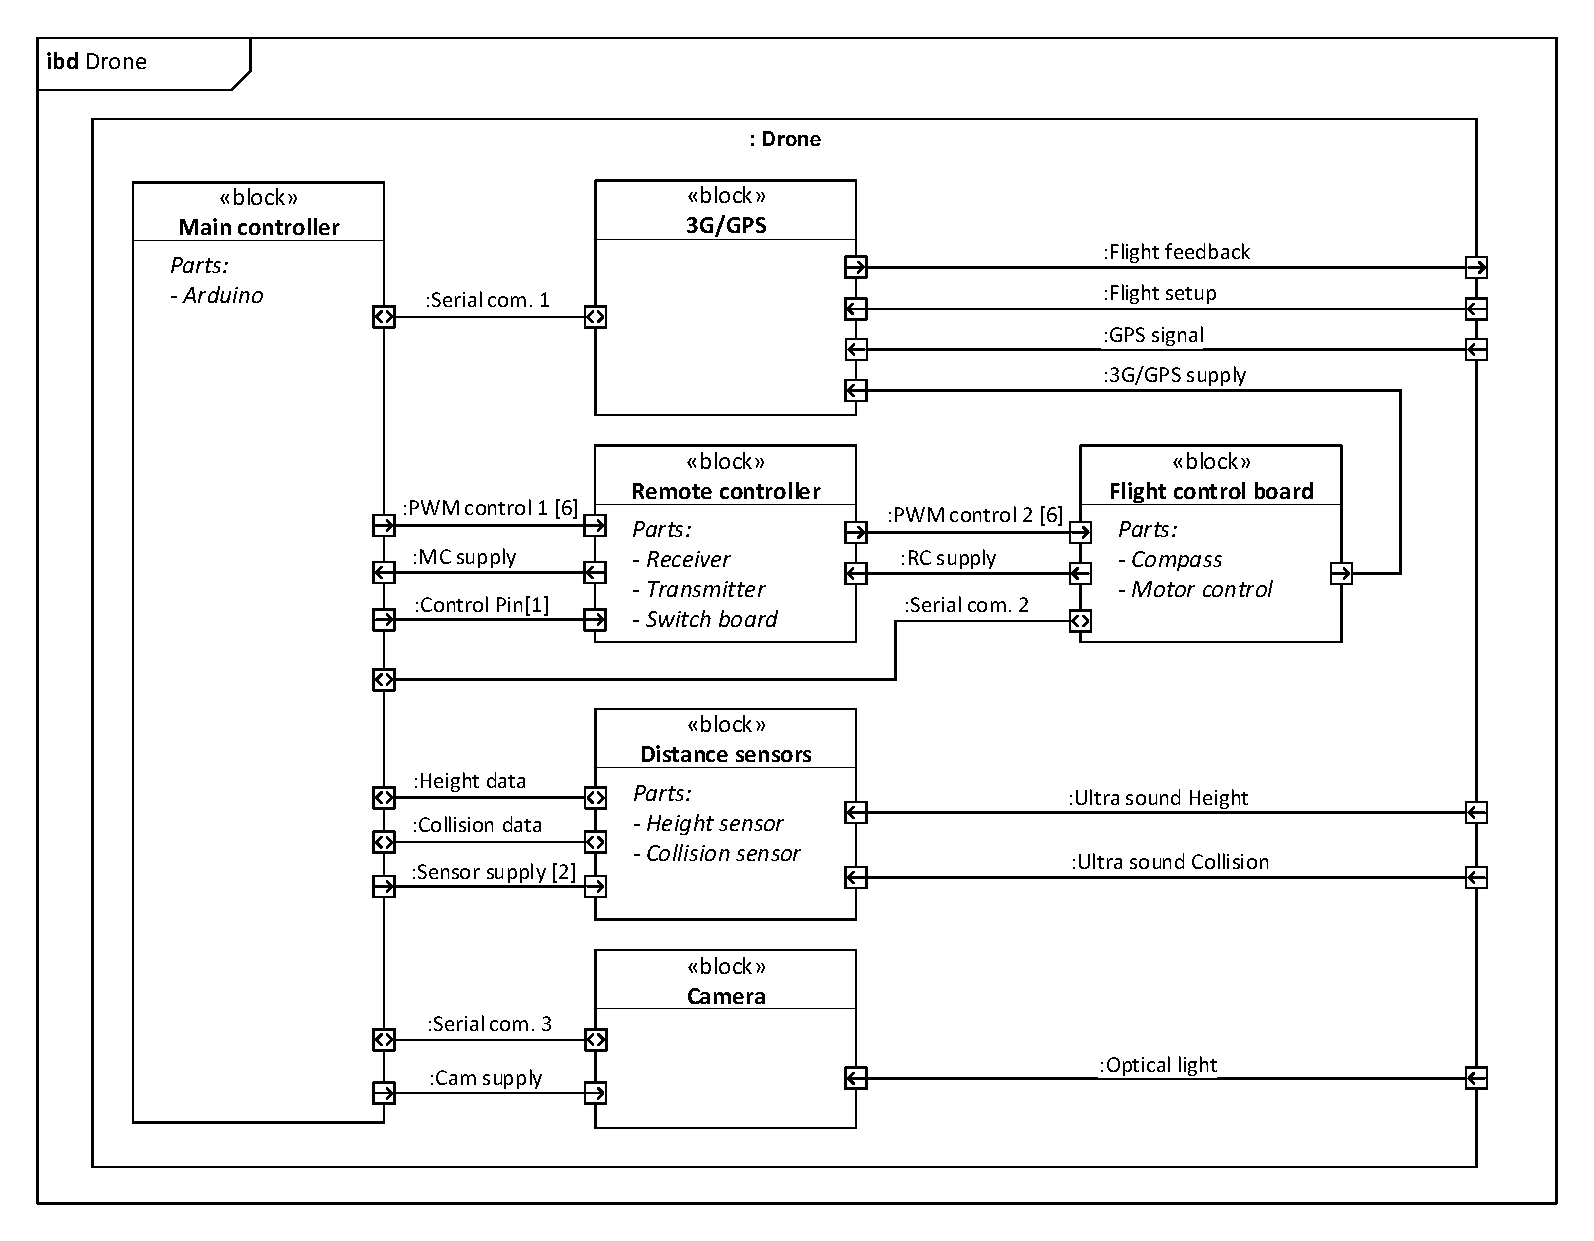
\includegraphics[width=1\textwidth]{Billeder/IBD/ibd2_drone.pdf}
\vspace{-0.5cm}
\caption{\textbf{ibd} - drone}
\label{fig:ibd_drone}
\end{figure}

\begin{table}[H]
	\centering
		\begin{tabular}	{|p{3.1 cm}|p{5.2 cm}|p{2.3 cm}|p{2.3 cm}|}  
								
		\hline
			\textbf{Signal navn} 	& \textbf{Signal beskrivelse}		& \textbf{Out} 		& \textbf{In}     \\ \hline
			Flight feedback		& Handshake og billeder				& 3G/GPS module.				& Webserver.	\\ \hline
			Flight setup		& Handshake \& Flyveopsætning  		& Webserver.			& 3G/GPS \newline module.	\\ \hline
			GPS signal	 		& GPS signal						& GPS-satellitter		& 3G/GPS \newline module.	\\ \hline			
			3G/GPS supply		& 5V DC							 	& Arduino	& 3G/GPS \newline module.    \\ \hline
			Serial com. 1		& RX / TX signaler. \newline Styrer 3G modul.& Main \newline controller. 		& 3G/GPS \newline module.    \\ \hline
			
			
			PWM control 1 [6]	& 244 Hz 6 kanals signal. Duty \newline cycle 25-50\%. Periode på 4ms	& Main \newline controller.	& Remoto \newline controller.	\\ \hline
			MC supply		& 5V DC							 	& Flight \newline control. 	& Main \newline controller    \\ \hline
			Control pin [1]		& Skifter mellem 5V og 0V							 	& Main \newline controller	& Remoto \newline  controller.    \\ \hline
			
			PWM control 2 [6]	& 50 Hz 6 kanals signal. Duty \newline cycle 5-10\%. Periode på 20ms	& Remote \newline controller.	& Flight \newline control.	\\ \hline		RC supply			& 5V DC							 	& Flight control	& Remote \newline controller.    \\ \hline
			Serial com. 2		& RX / TX signaler. \newline Aflæsning kompas. & Main \newline controller.	& Flight \newline control.	\\ \hline 	
			
			Height data.		& Trigger \& echo signal der \newline indikerer afstanden. 	& Main \newline controller.	& Distance \newline sensors.	\\ \hline
			Collision data.		& Trigger \& echo signal der \newline indikerer afstanden. 	& Main \newline controller.	& Distance \newline sensors.  \\ \hline
			Sensor supply [2]	& 5V DC.	& Main \newline controller. & Distance \newline sensors.	\\ \hline
			Ultra sound \newline Height			& Afstand vha. ultralyd. \newline (8 bursts af 40kHz) 	& Distance \newline sensor.	& Omgivelserne.	\\ \hline 
			Ultra sound \newline	Collision		& Afstand vha. ultralyd. \newline (8 bursts af 40kHz) 	& Distance \newline sensor.	& Omgivelserne.	\\ \hline 			
				
			Serial com. 3		& RX / TX signal. \newline Styrer kamera.	& Main \newline controller.	& Camera.	\\ \hline
			Cam supply			& 5V DC 	& Main \newline controller.	& Camera.	\\ \hline
			Optical light		& Kamera billede. 	& Camera.	& Omgivelserne.	\\ \hline	
			
		\end{tabular}
	\caption{Forbindelser til: \textbf{Ibd} - drone}
	\label{tab:IBDdrone}
\end{table}

